\newpage
\subsection{Diseño de interfaces de la plataforma web (UI/UX)}

El desarrollo de la plataforma web está orientado a proveer tanto al experto de campo como a los administradores un entorno eficiente para el análisis forestal y la gestión del sistema. El diseño visual y la experiencia de usuario (UX) se estructuraron buscando mantener una alta coherencia e identidad visual con la aplicación móvil. Por este motivo, se implementó la misma paleta cromática (enfocada en tonos de naturaleza, tierra y acentos de alerta), logrando consistencia bajo los lineamientos de \textit{Material Design}.

\subsubsection{Módulo de Autenticación}

El punto de entrada al sistema web requiere un control de acceso estricto. Se diseñaron interfaces minimalistas para el inicio de sesión y la recuperación de credenciales, asegurando que el usuario pueda autenticarse rápidamente o restablecer su acceso sin fricción.



% Agrega esto en tu preámbulo o justo antes de las imágenes
\setlength{\fboxsep}{0pt} % Espacio entre borde e imagen
\setlength{\fboxrule}{1pt} % Grosor del borde negro

% Espacio para Maqueta de Login / Recuperación
\begin{figure}[H]
    \centering
    \fbox{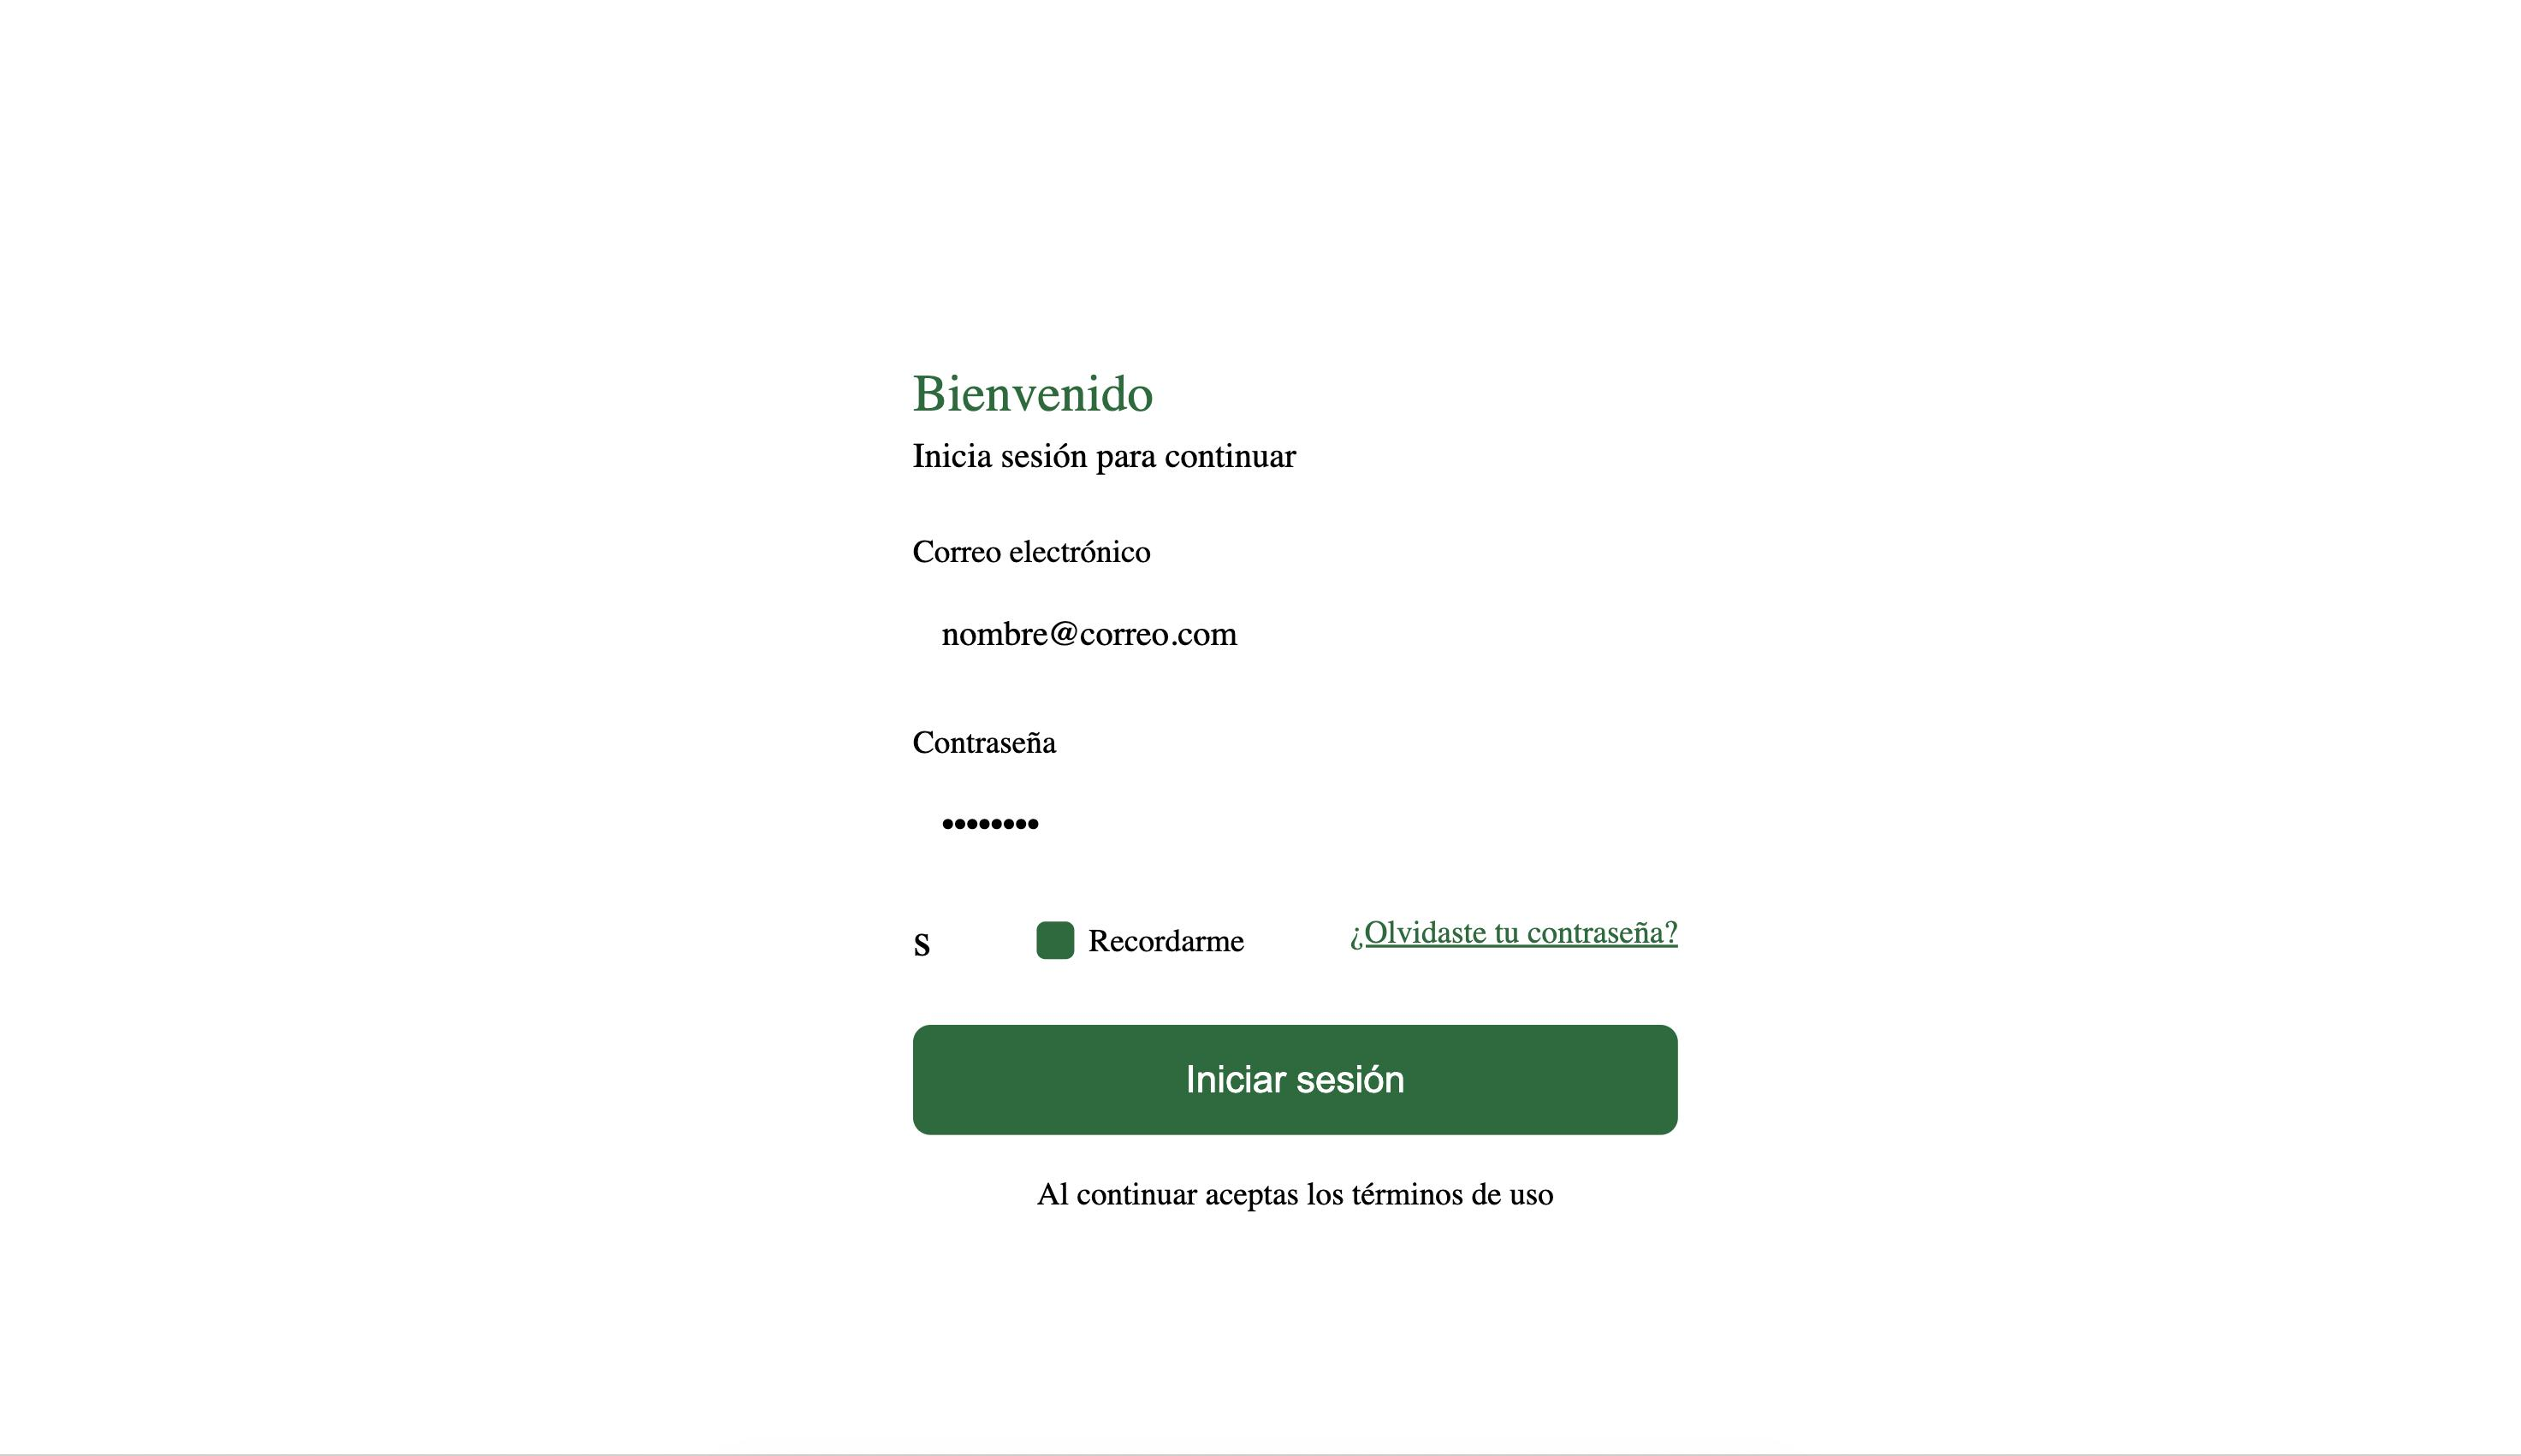
\includegraphics[width=0.8\textwidth]{images/Pantallas/Web/login.jpeg}}
    \caption{Maqueta de inicio de sesión.}
    \label{fig:web_auth}
\end{figure}

\begin{figure}[H]
    \centering
    \fbox{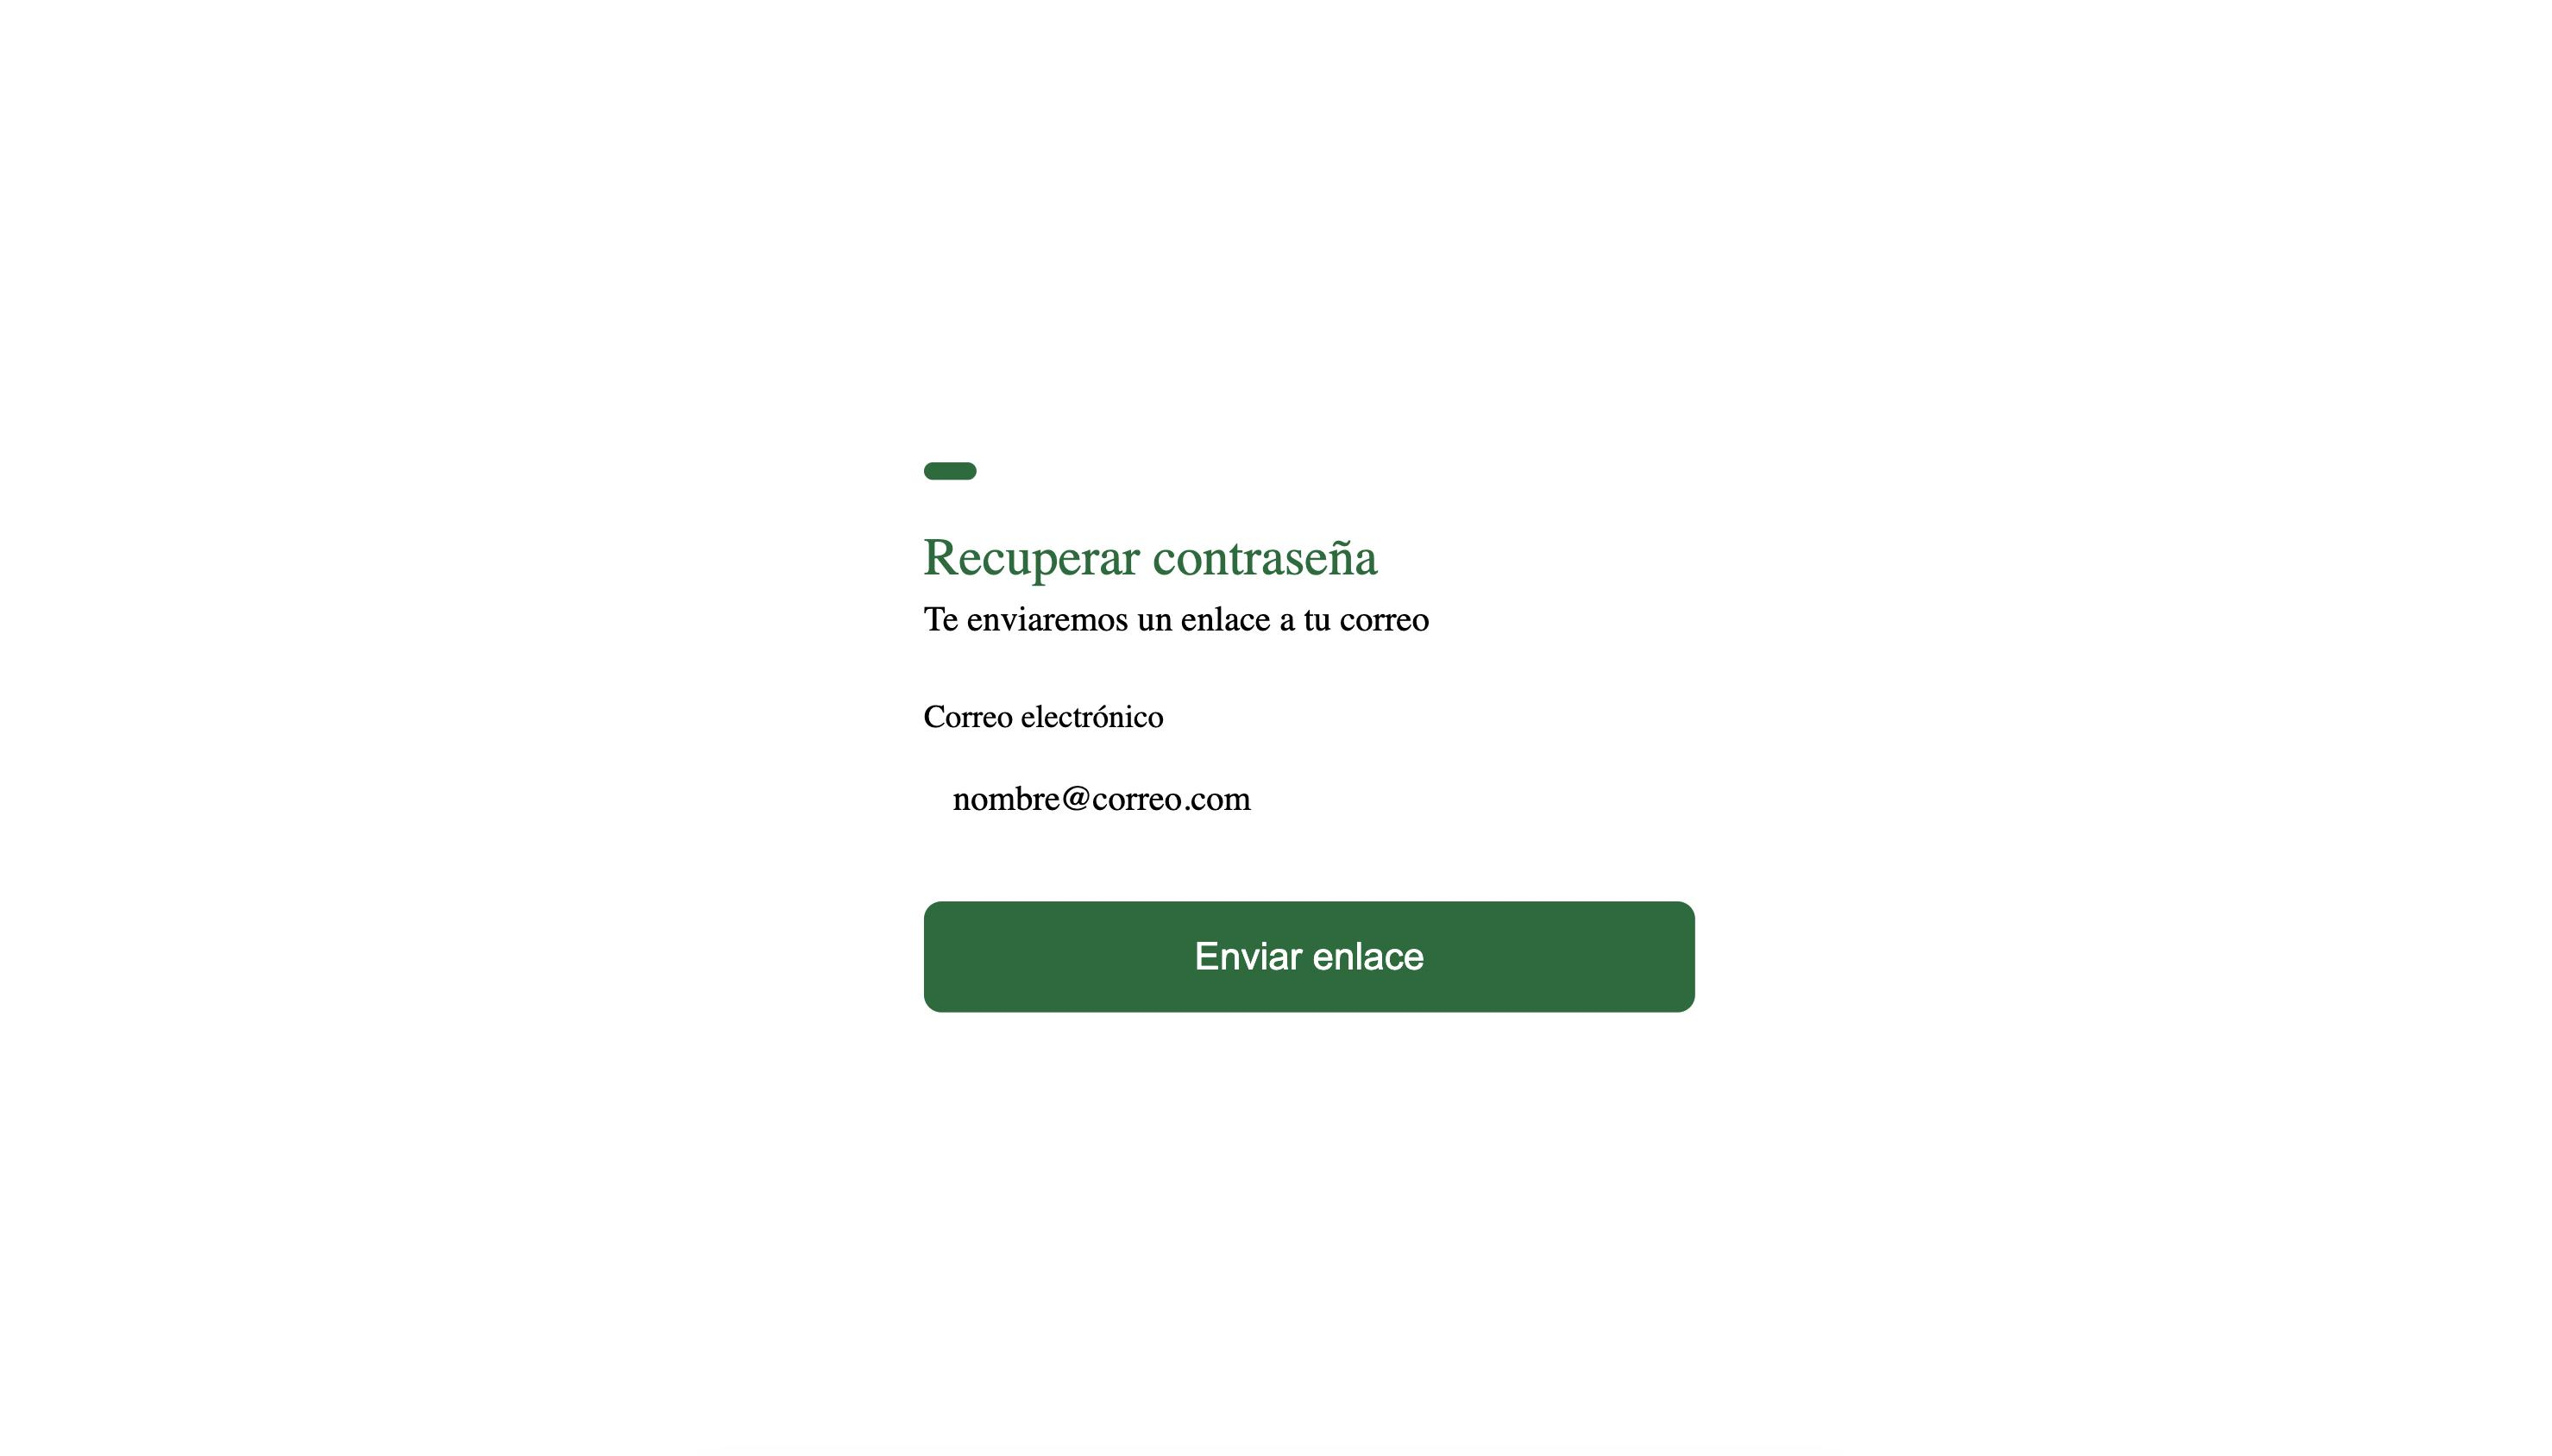
\includegraphics[width=0.8\textwidth]{images/Pantallas/Web/recuperar.jpeg}}
    \caption{Maqueta de recuperacion de contraseña.}
    \label{fig:web_auth1}
\end{figure}

\begin{figure}[H]
    \centering
    \fbox{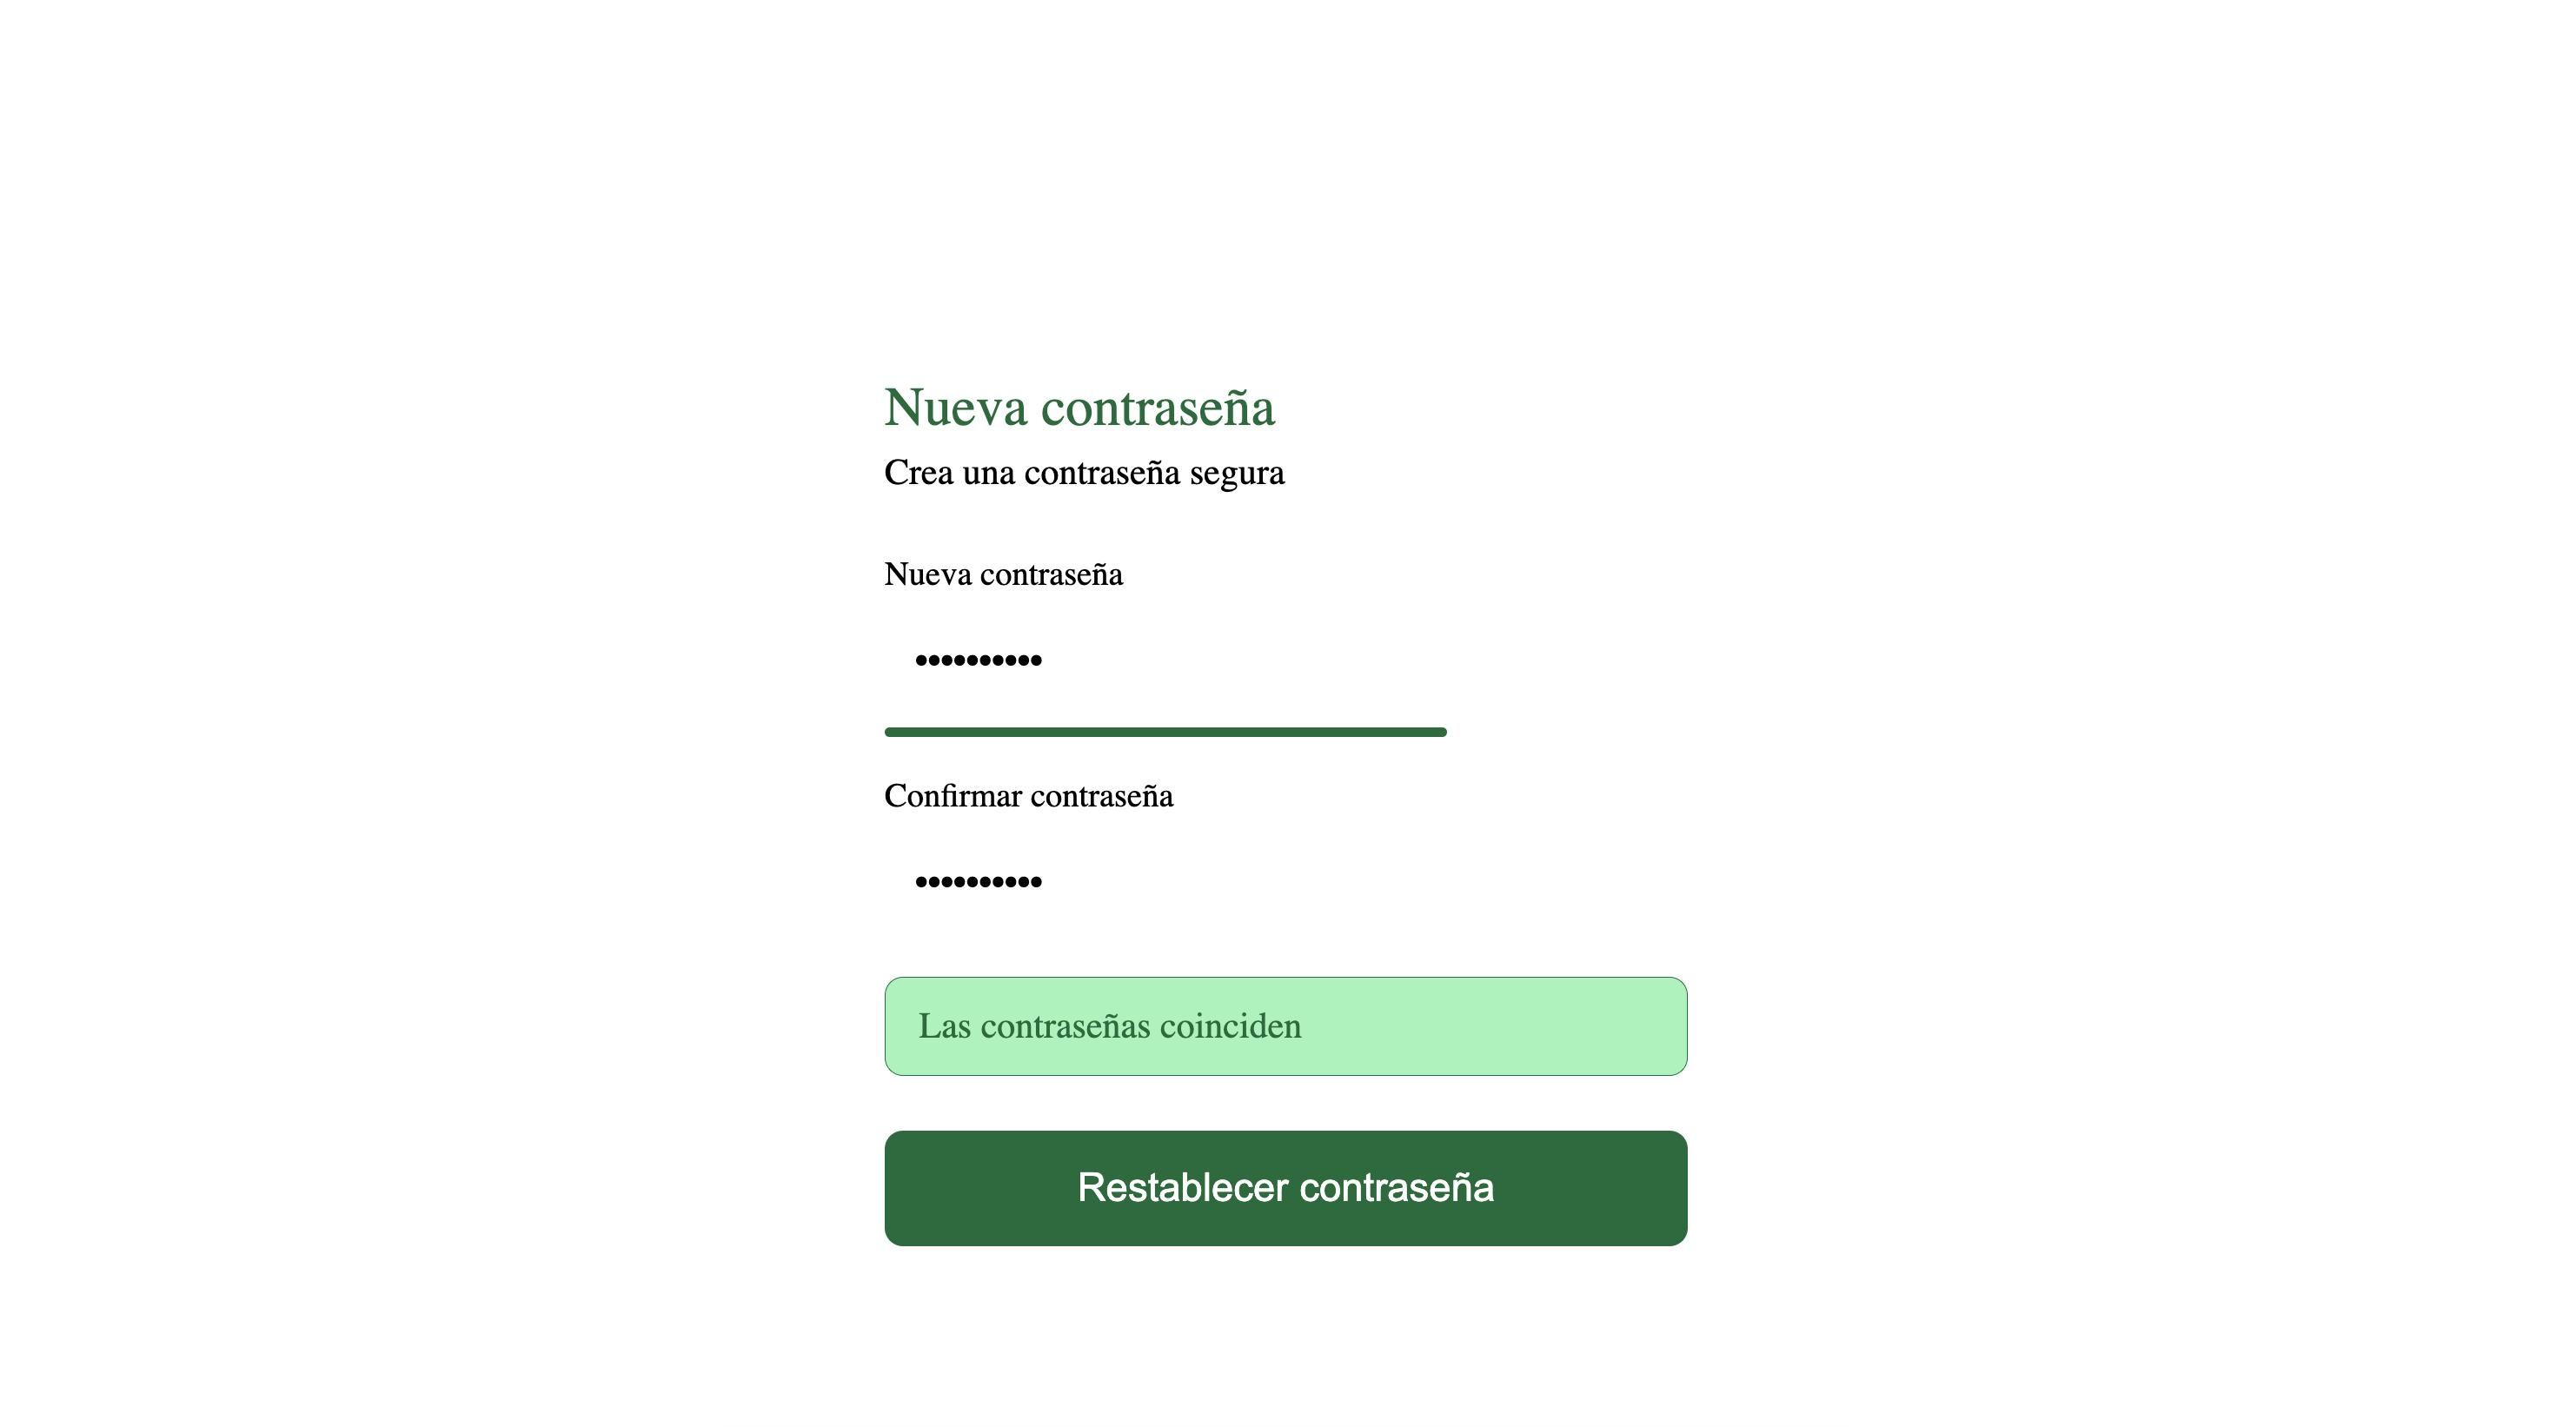
\includegraphics[width=0.8\textwidth]{images/Pantallas/Web/nueva.jpeg}}
    \caption{Maqueta de nueva contraseña.}
    \label{fig:web_auth2}
\end{figure}


\subsubsection{Panel administrativo y gestión de usuarios}

Para el rol de Administrador, se definió un módulo de control interno. Esta interfaz permite la gestión integral del sistema mediante vistas tabulares y formularios modales para la creación, edición y desactivación de cuentas de usuario, así como la asignación de roles y la gestión de los dispositivos de escaneo vinculados a cada cuenta.

\begin{figure}[H]
    \centering
    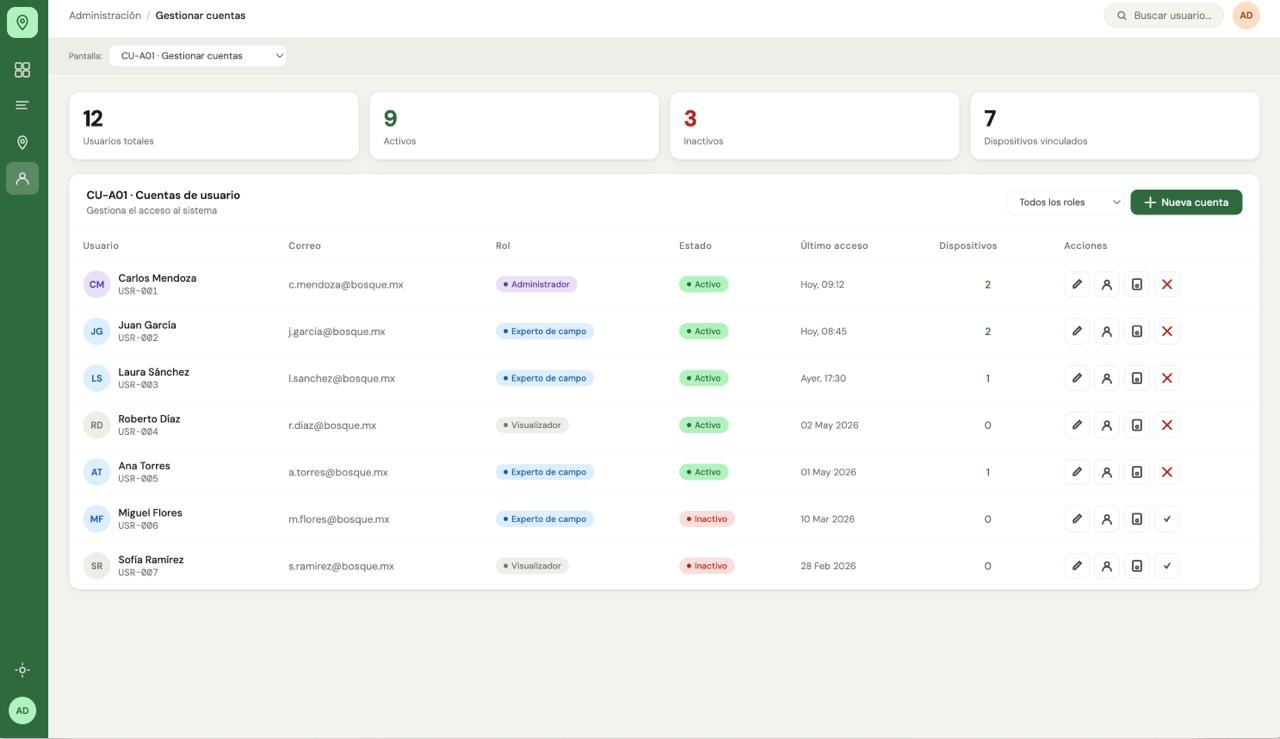
\includegraphics[width=1\textwidth]{images/Pantallas/Web/gestionar.jpeg}
    \caption{CU-A01: Gestión general de cuentas de usuario.}
    \label{fig:web_gestionar}
\end{figure}

\begin{figure}[H]
    \centering
    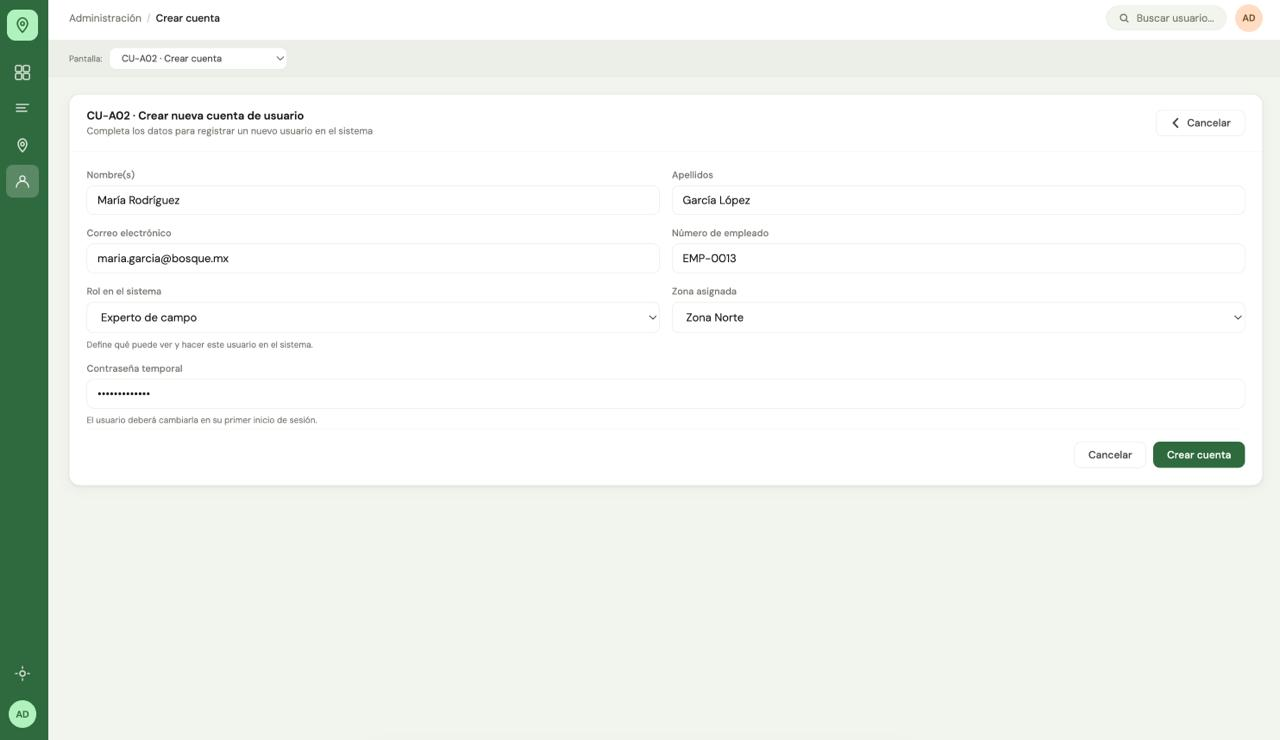
\includegraphics[width=1\textwidth]{images/Pantallas/Web/crear_cuenta.jpeg}
    \caption{CU-A02: Creación de nueva cuenta de usuario.}
    \label{fig:web_crear_cuenta}
\end{figure}

\begin{figure}[H]
    \centering
    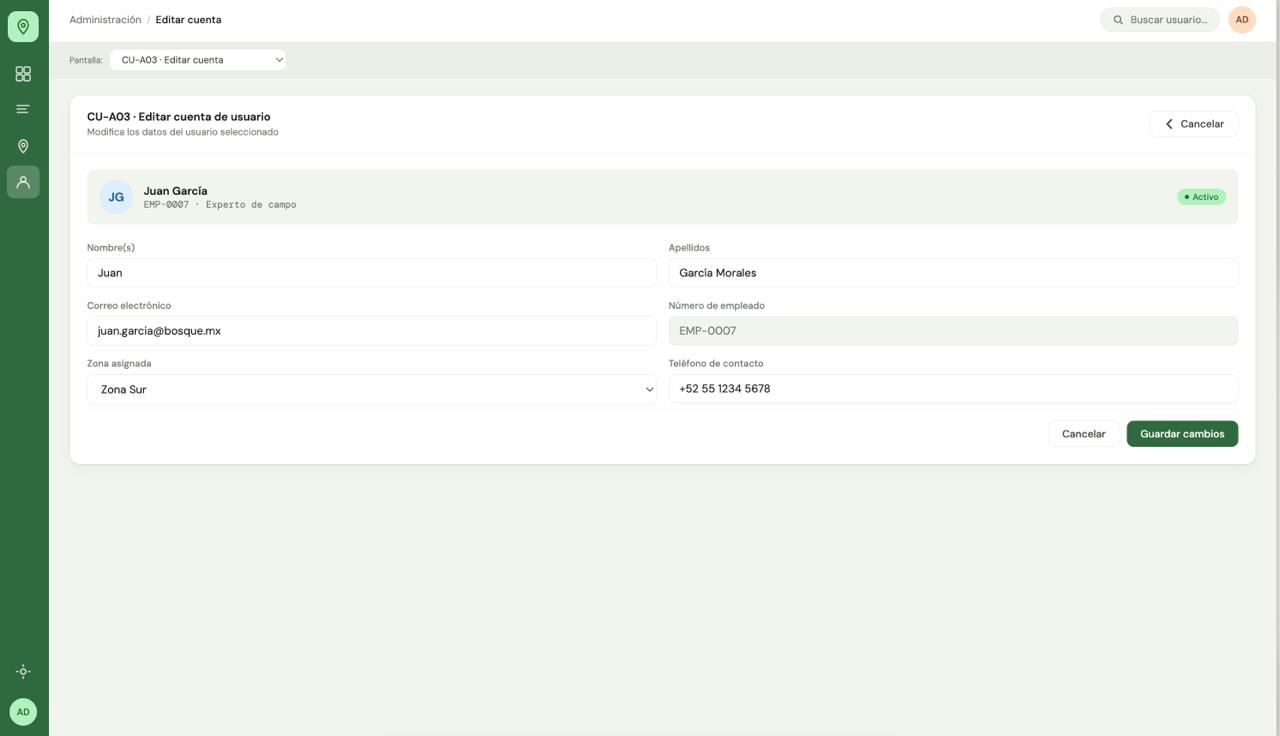
\includegraphics[width=1\textwidth]{images/Pantallas/Web/editar_cuenta.jpeg}
    \caption{CU-A03: Edición de datos de cuenta de usuario.}
    \label{fig:web_editar_cuenta}
\end{figure}

\begin{figure}[H]
    \centering
    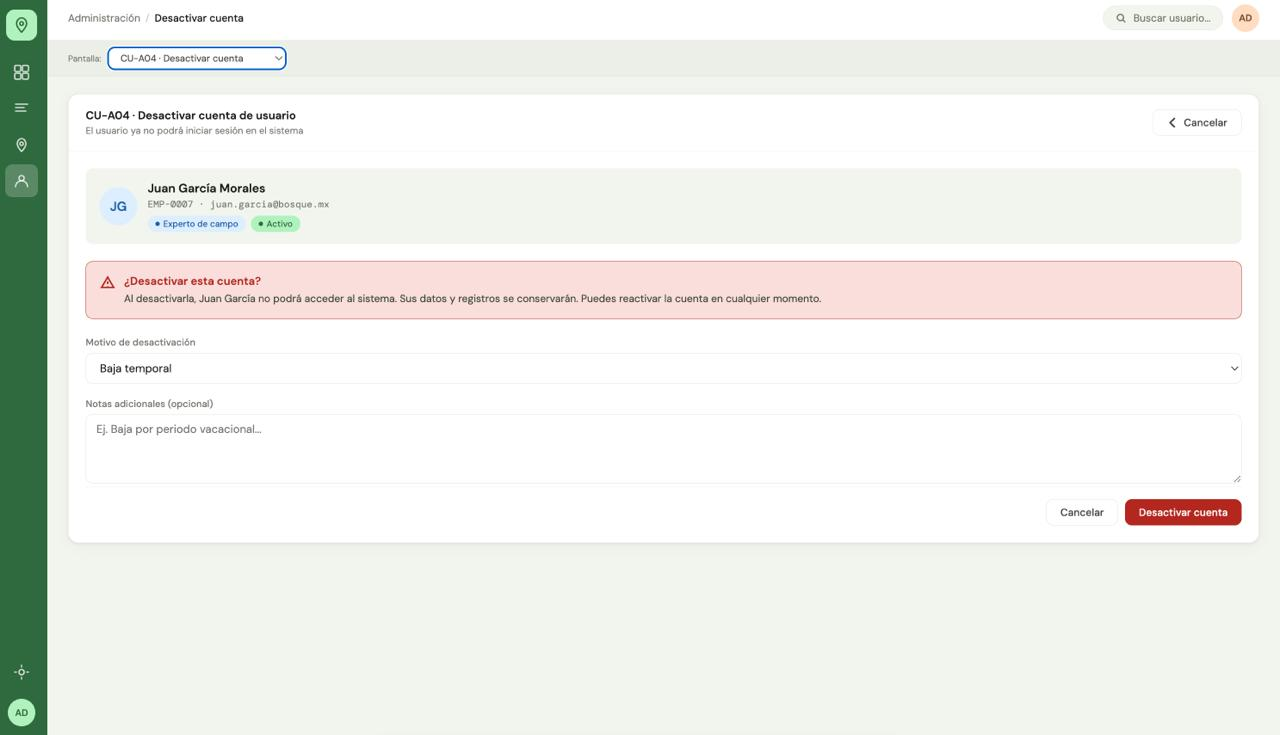
\includegraphics[width=1\textwidth]{images/Pantallas/Web/desactivar.jpeg}
    \caption{CU-A04: Desactivación de cuenta de usuario.}
    \label{fig:web_desactivar}
\end{figure}

\begin{figure}[H]
    \centering
    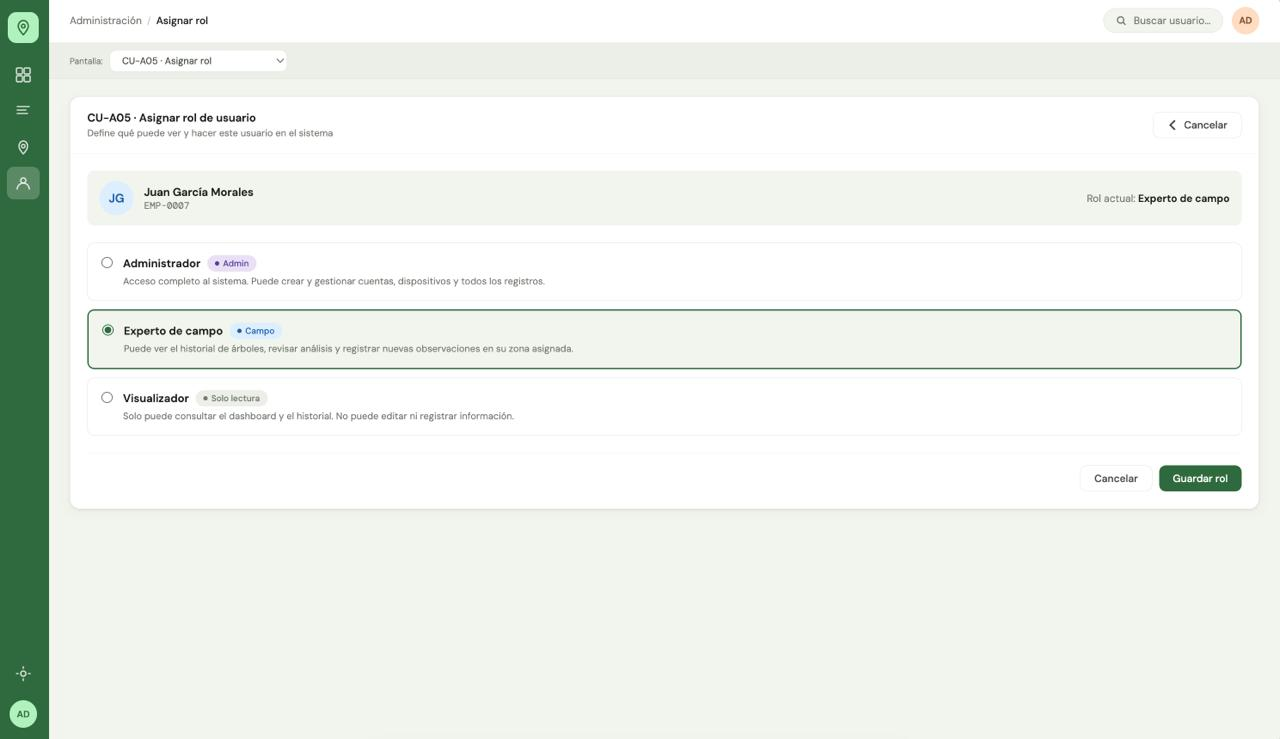
\includegraphics[width=1\textwidth]{images/Pantallas/Web/asignar_rol.jpeg}
    \caption{CU-A05: Asignación de rol a cuenta de usuario.}
    \label{fig:web_asignar_rol}
\end{figure}

\begin{figure}[H]
    \centering
    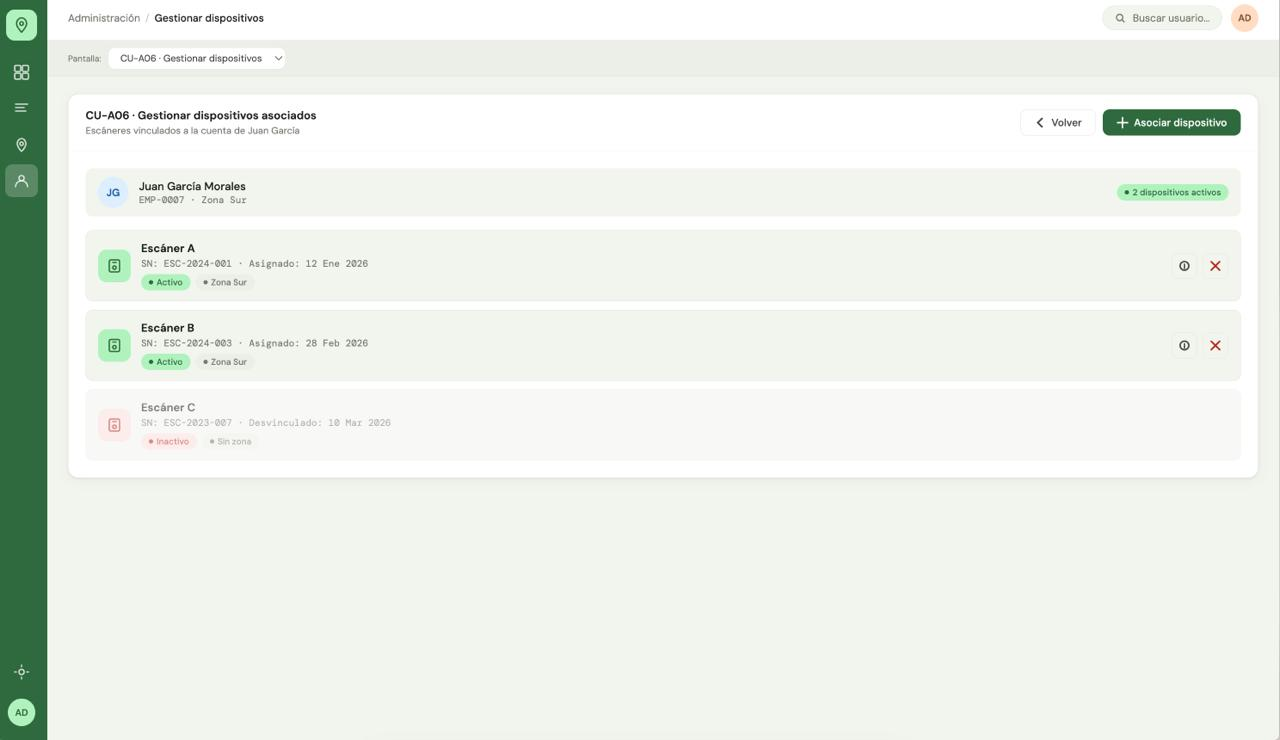
\includegraphics[width=1\textwidth]{images/Pantallas/Web/gestionar_dispositivos.jpeg}
    \caption{CU-A06: Gestión de dispositivos asociados a una cuenta.}
    \label{fig:web_gestionar_dispositivos}
\end{figure}

\begin{figure}[H]
    \centering
    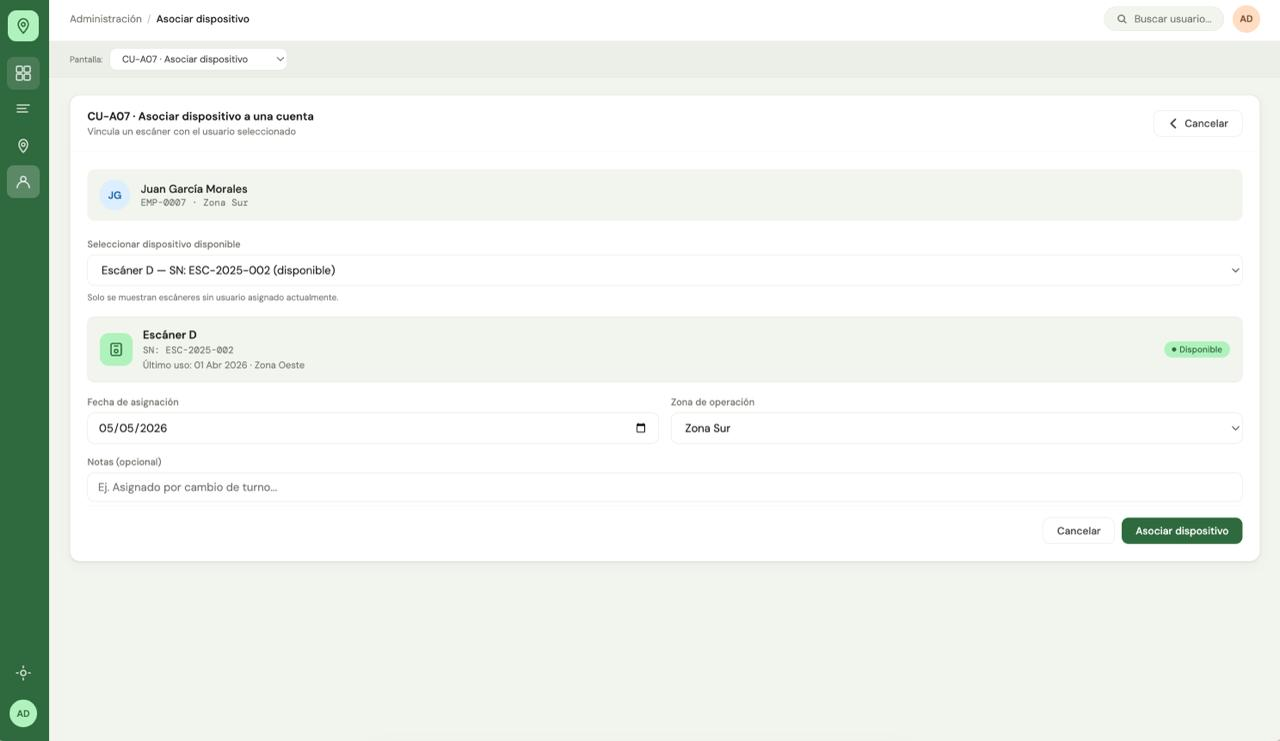
\includegraphics[width=1\textwidth]{images/Pantallas/Web/asociar.jpeg}
    \caption{CU-A07: Asociación de dispositivo escáner a una cuenta de usuario.}
    \label{fig:web_asociar}
\end{figure}

\begin{figure}[H]
    \centering
    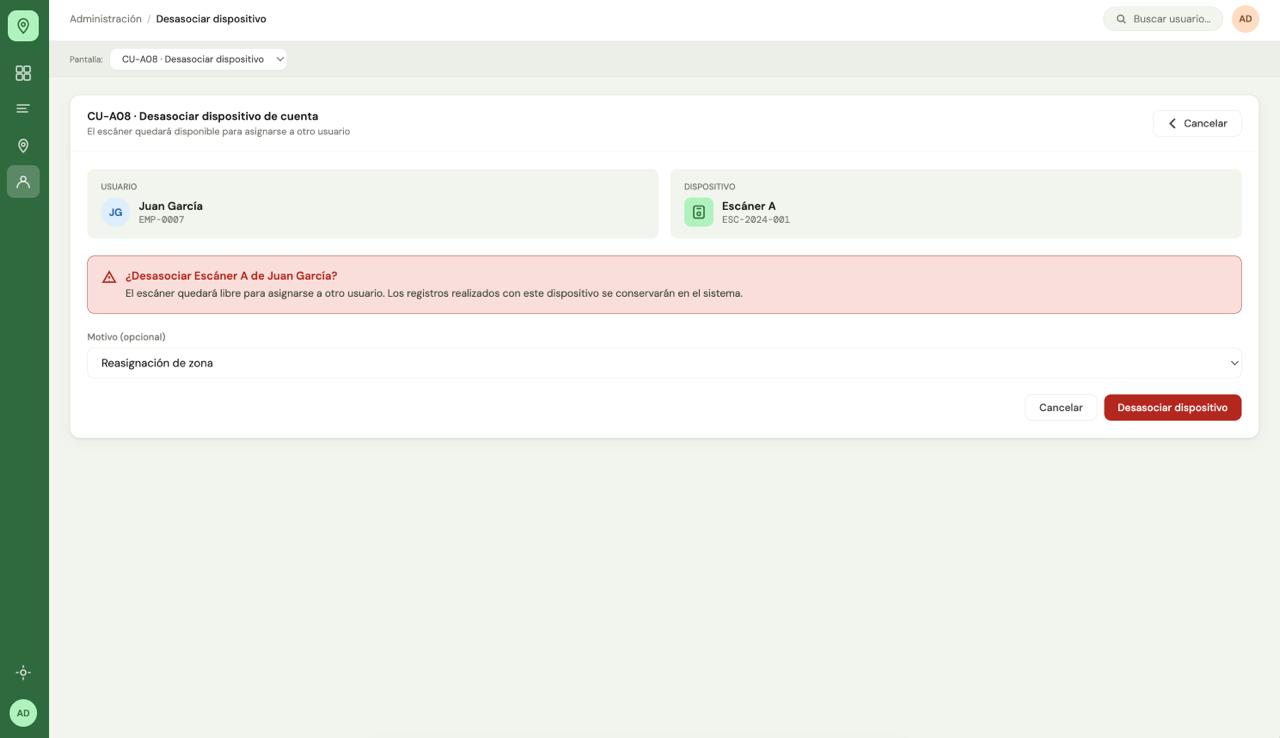
\includegraphics[width=1\textwidth]{images/Pantallas/Web/desasociar.jpeg}
    \caption{CU-A08: Desasociación de dispositivo escáner de una cuenta de usuario.}
    \label{fig:web_desasociar}
\end{figure}

\subsubsection{Dashboard y flujo de navegación (Experto de Campo)}

El flujo de navegación para el experto de campo minimiza la cantidad de clics necesarios para acceder a la información crítica. Mediante un menú lateral (\textit{sidebar}) dinámico, el usuario puede transitar entre el resumen general, el historial de registros, el mapa interactivo y las estadísticas. 

% Espacio para Maqueta del Dashboard
\begin{figure}[H]
    \centering
    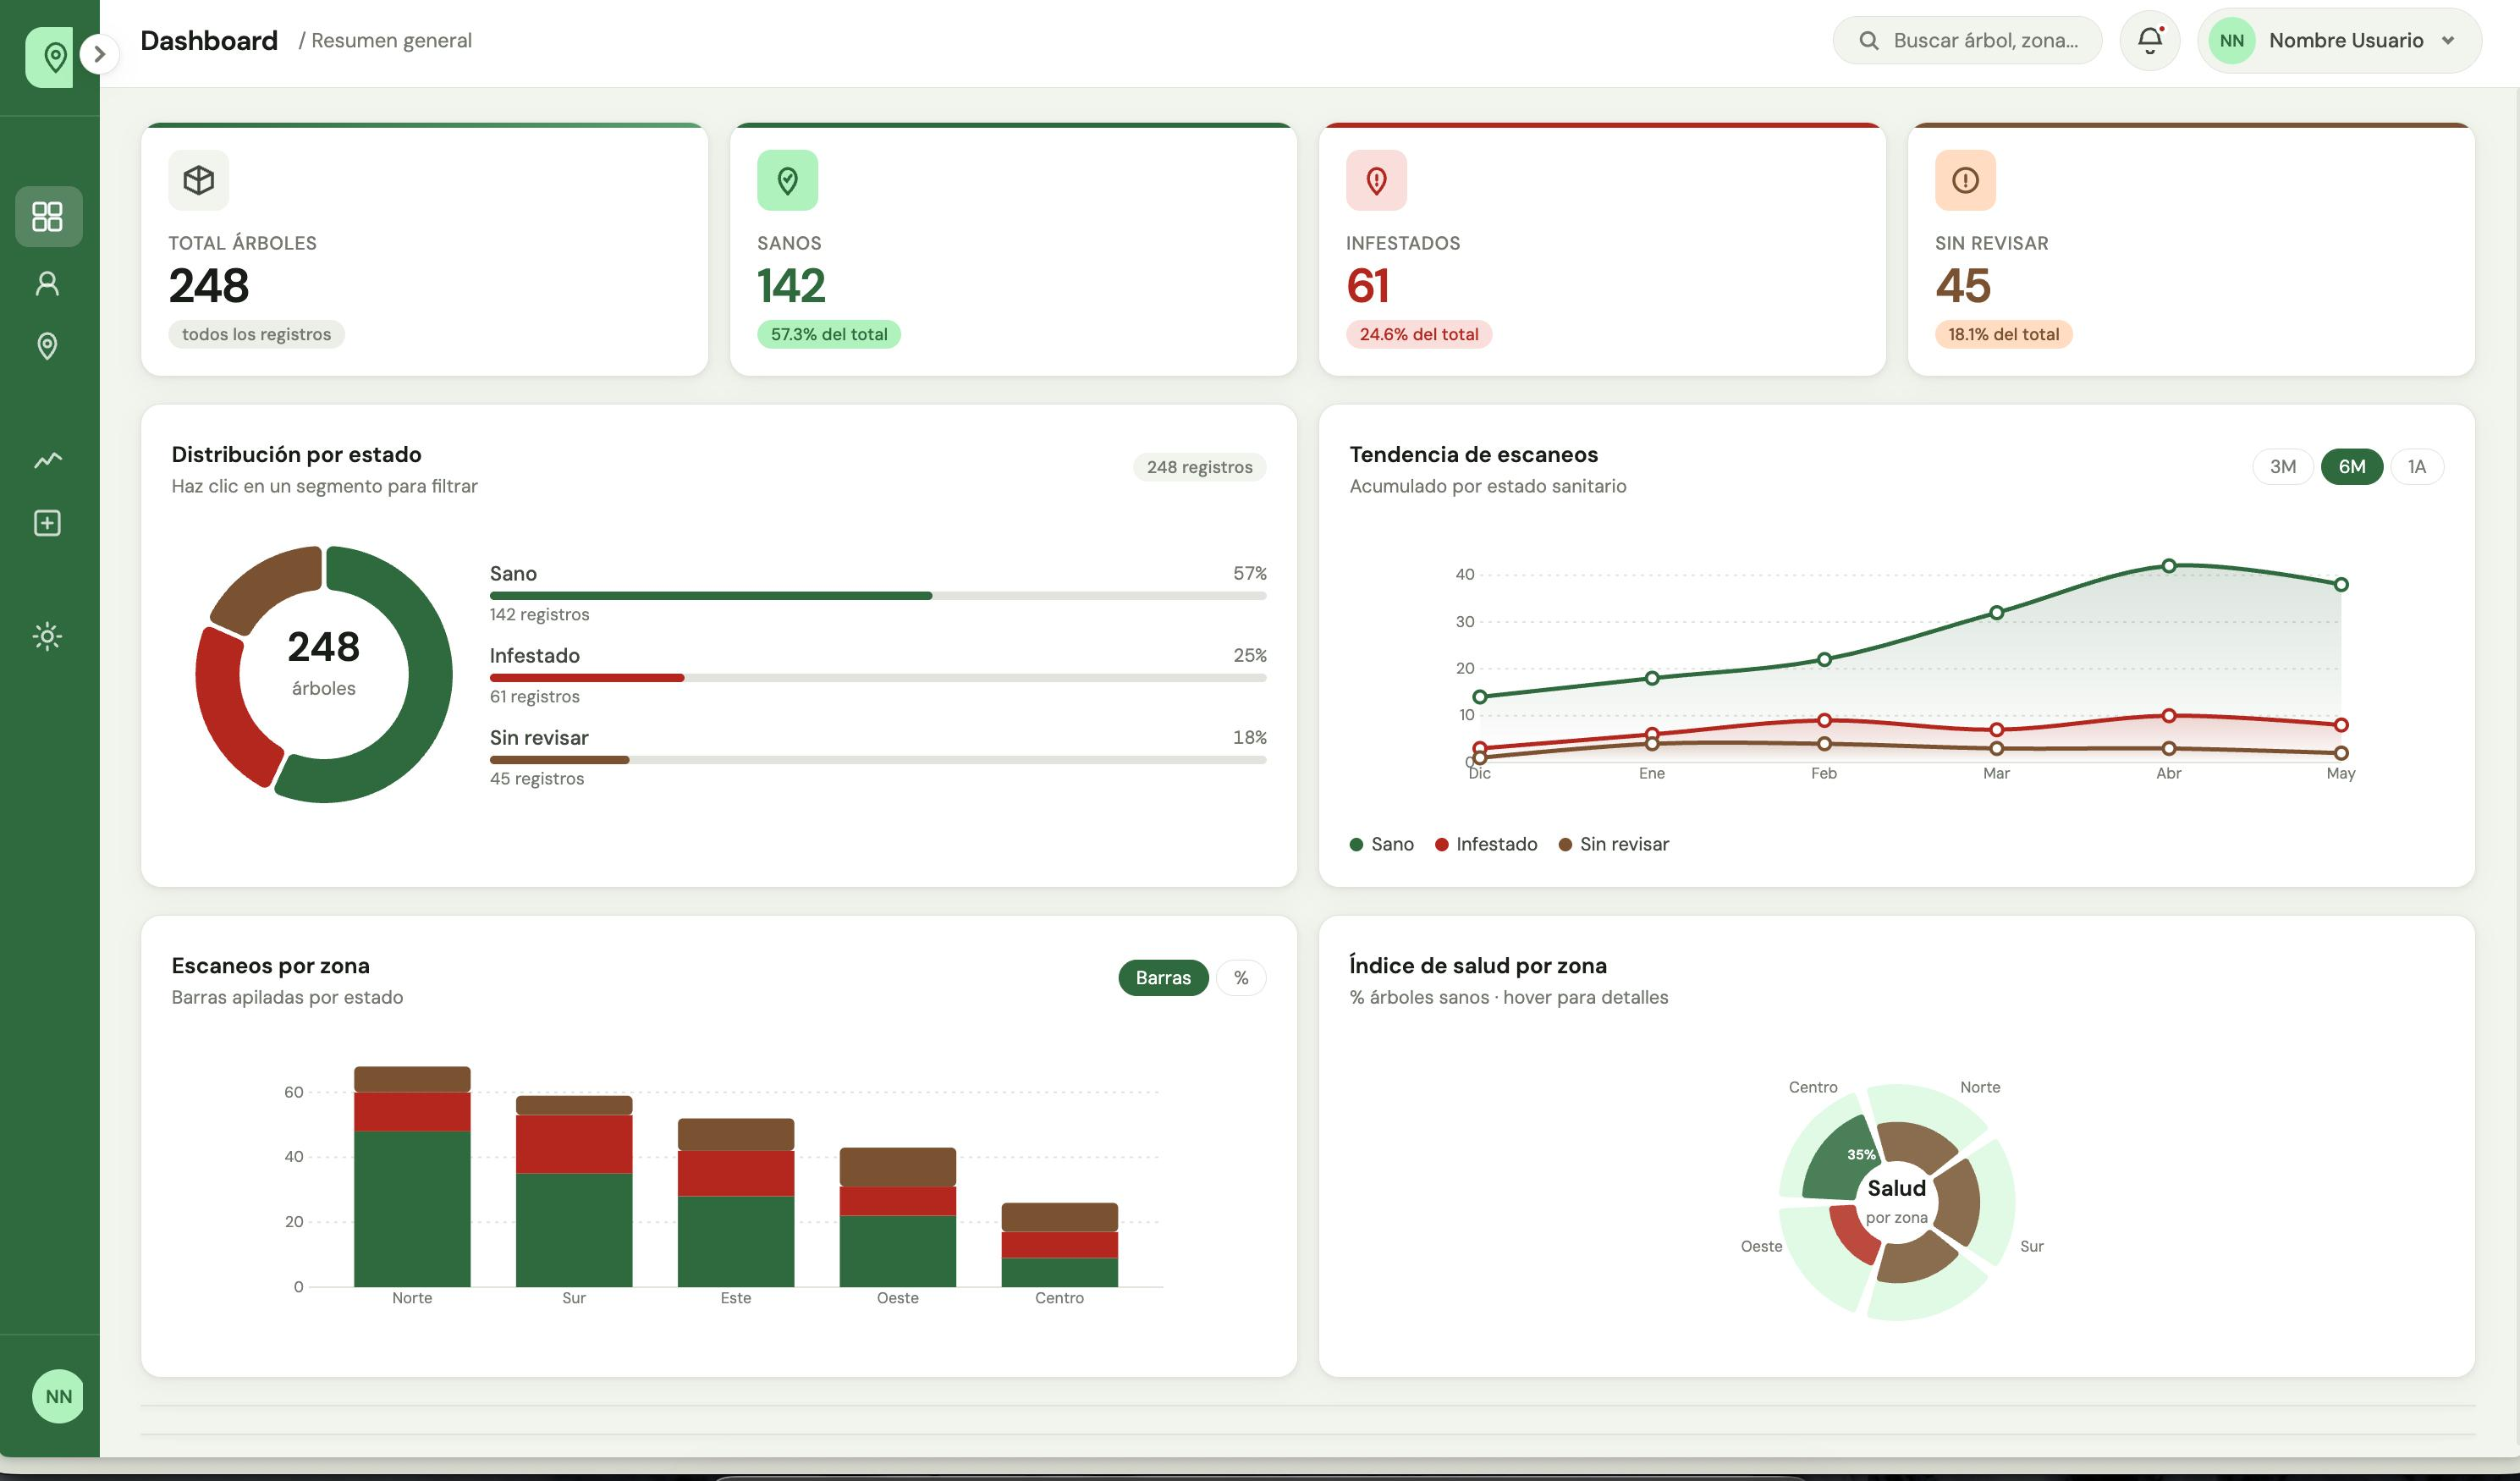
\includegraphics[width=1\textwidth]{images/Pantallas/Web/dashboard.jpeg}
    \caption{Interfaz del panel de resumen (Dashboard)}
    \label{fig:web_dashboard}
\end{figure}

\subsubsection{Análisis espacial e identificación de focos de infestación}

El análisis geoespacial es fundamental para la toma de decisiones ecológicas. Se diseñó una interfaz interactiva cartográfica que renderiza marcadores para cada árbol analizado. Este módulo cuenta con controles de filtrado dinámico que permiten aislar árboles sanos de aquellos en riesgo, facilitando la visualización inmediata de focos de infestación activos sobre el terreno.

% Espacio para Maqueta del Mapa
\begin{figure}[H]
    \centering
      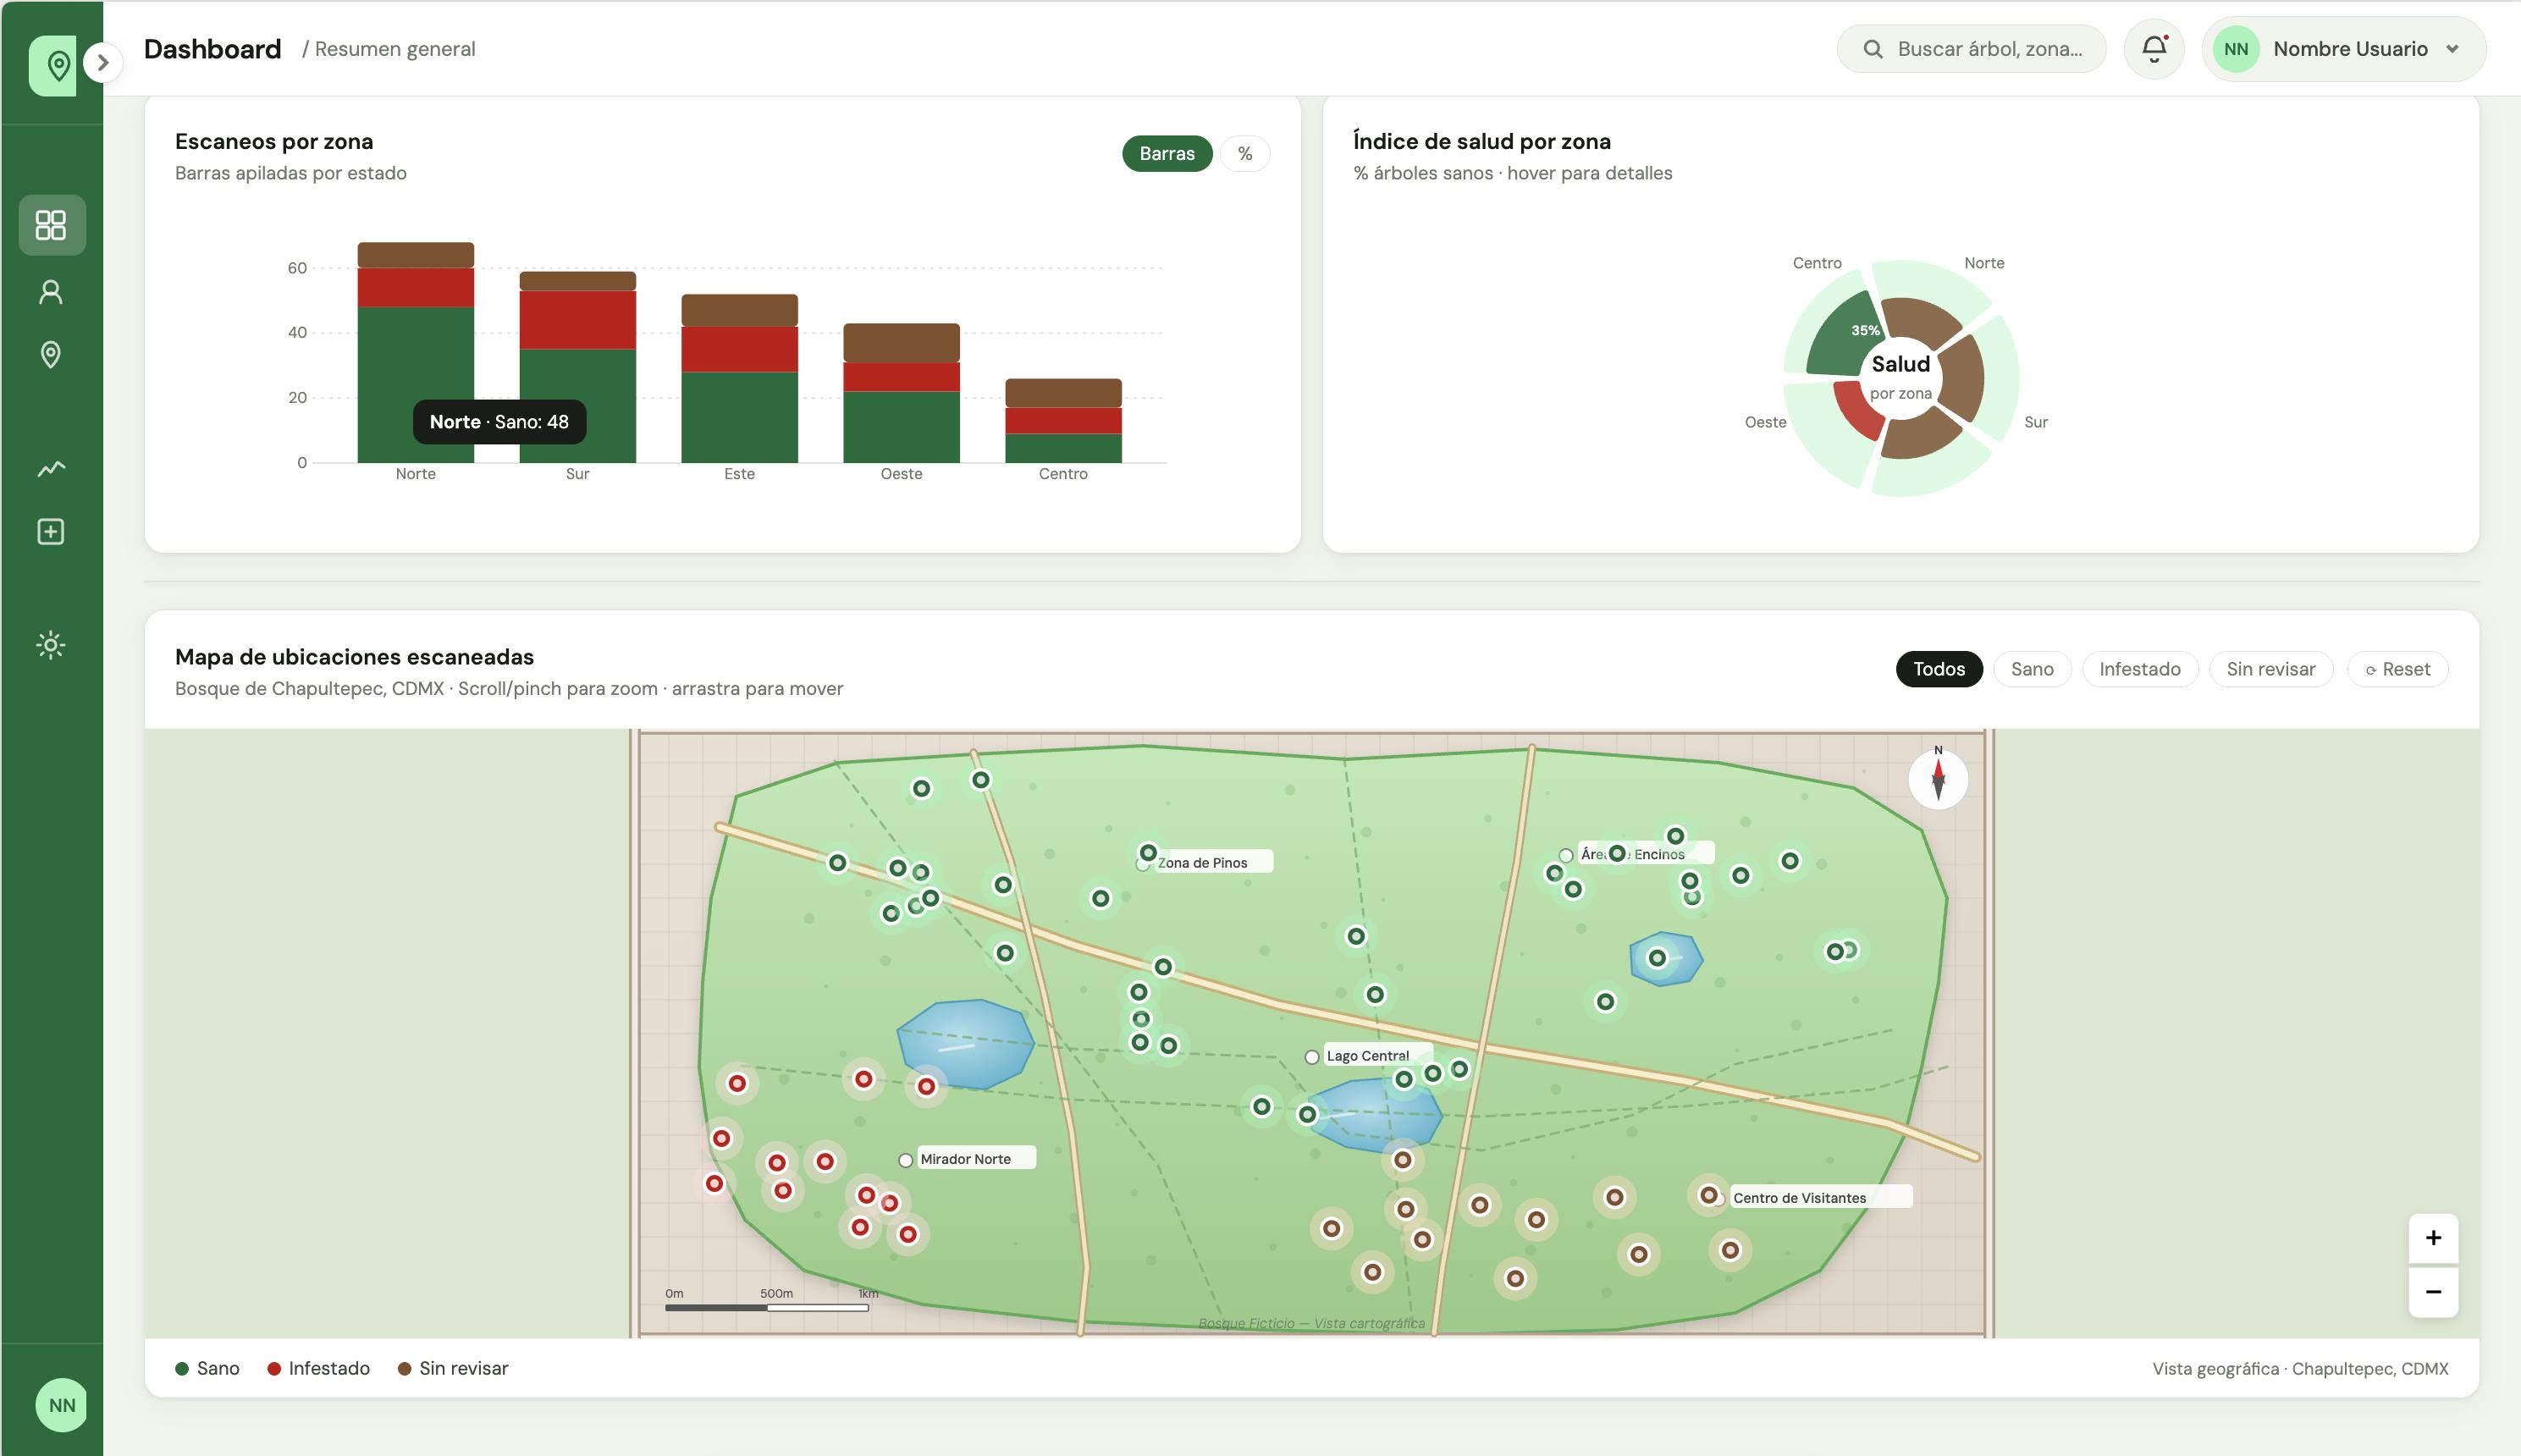
\includegraphics[width=1\textwidth]{images/Pantallas/Web/mapa.jpeg}
    \caption{Maqueta del mapa general de árboles y focos de infestación.}
    \label{fig:web_mapa}
\end{figure}

\subsubsection{Presentación de resultados analíticos (D3.js)}

Para presentar el alto volumen de datos provenientes de la base de datos PostgreSQL de manera analítica e intuitiva, se integró la librería \textit{D3.js}. Esta herramienta permite generar visualizaciones interactivas.

El sistema mapea los registros para renderizar gráficos de evolución temporal, distribución de especies y estados sanitarios, así como interfaces de análisis detallado por árbol (incluyendo evidencia fotográfica, resultados de clasificación neuronal y mapas de calor cromáticos), optimizando la interpretabilidad de los diagnósticos generados.

% Espacio para Maqueta de Historial Completo y Estadísticas
\begin{figure}[H]
    \centering
    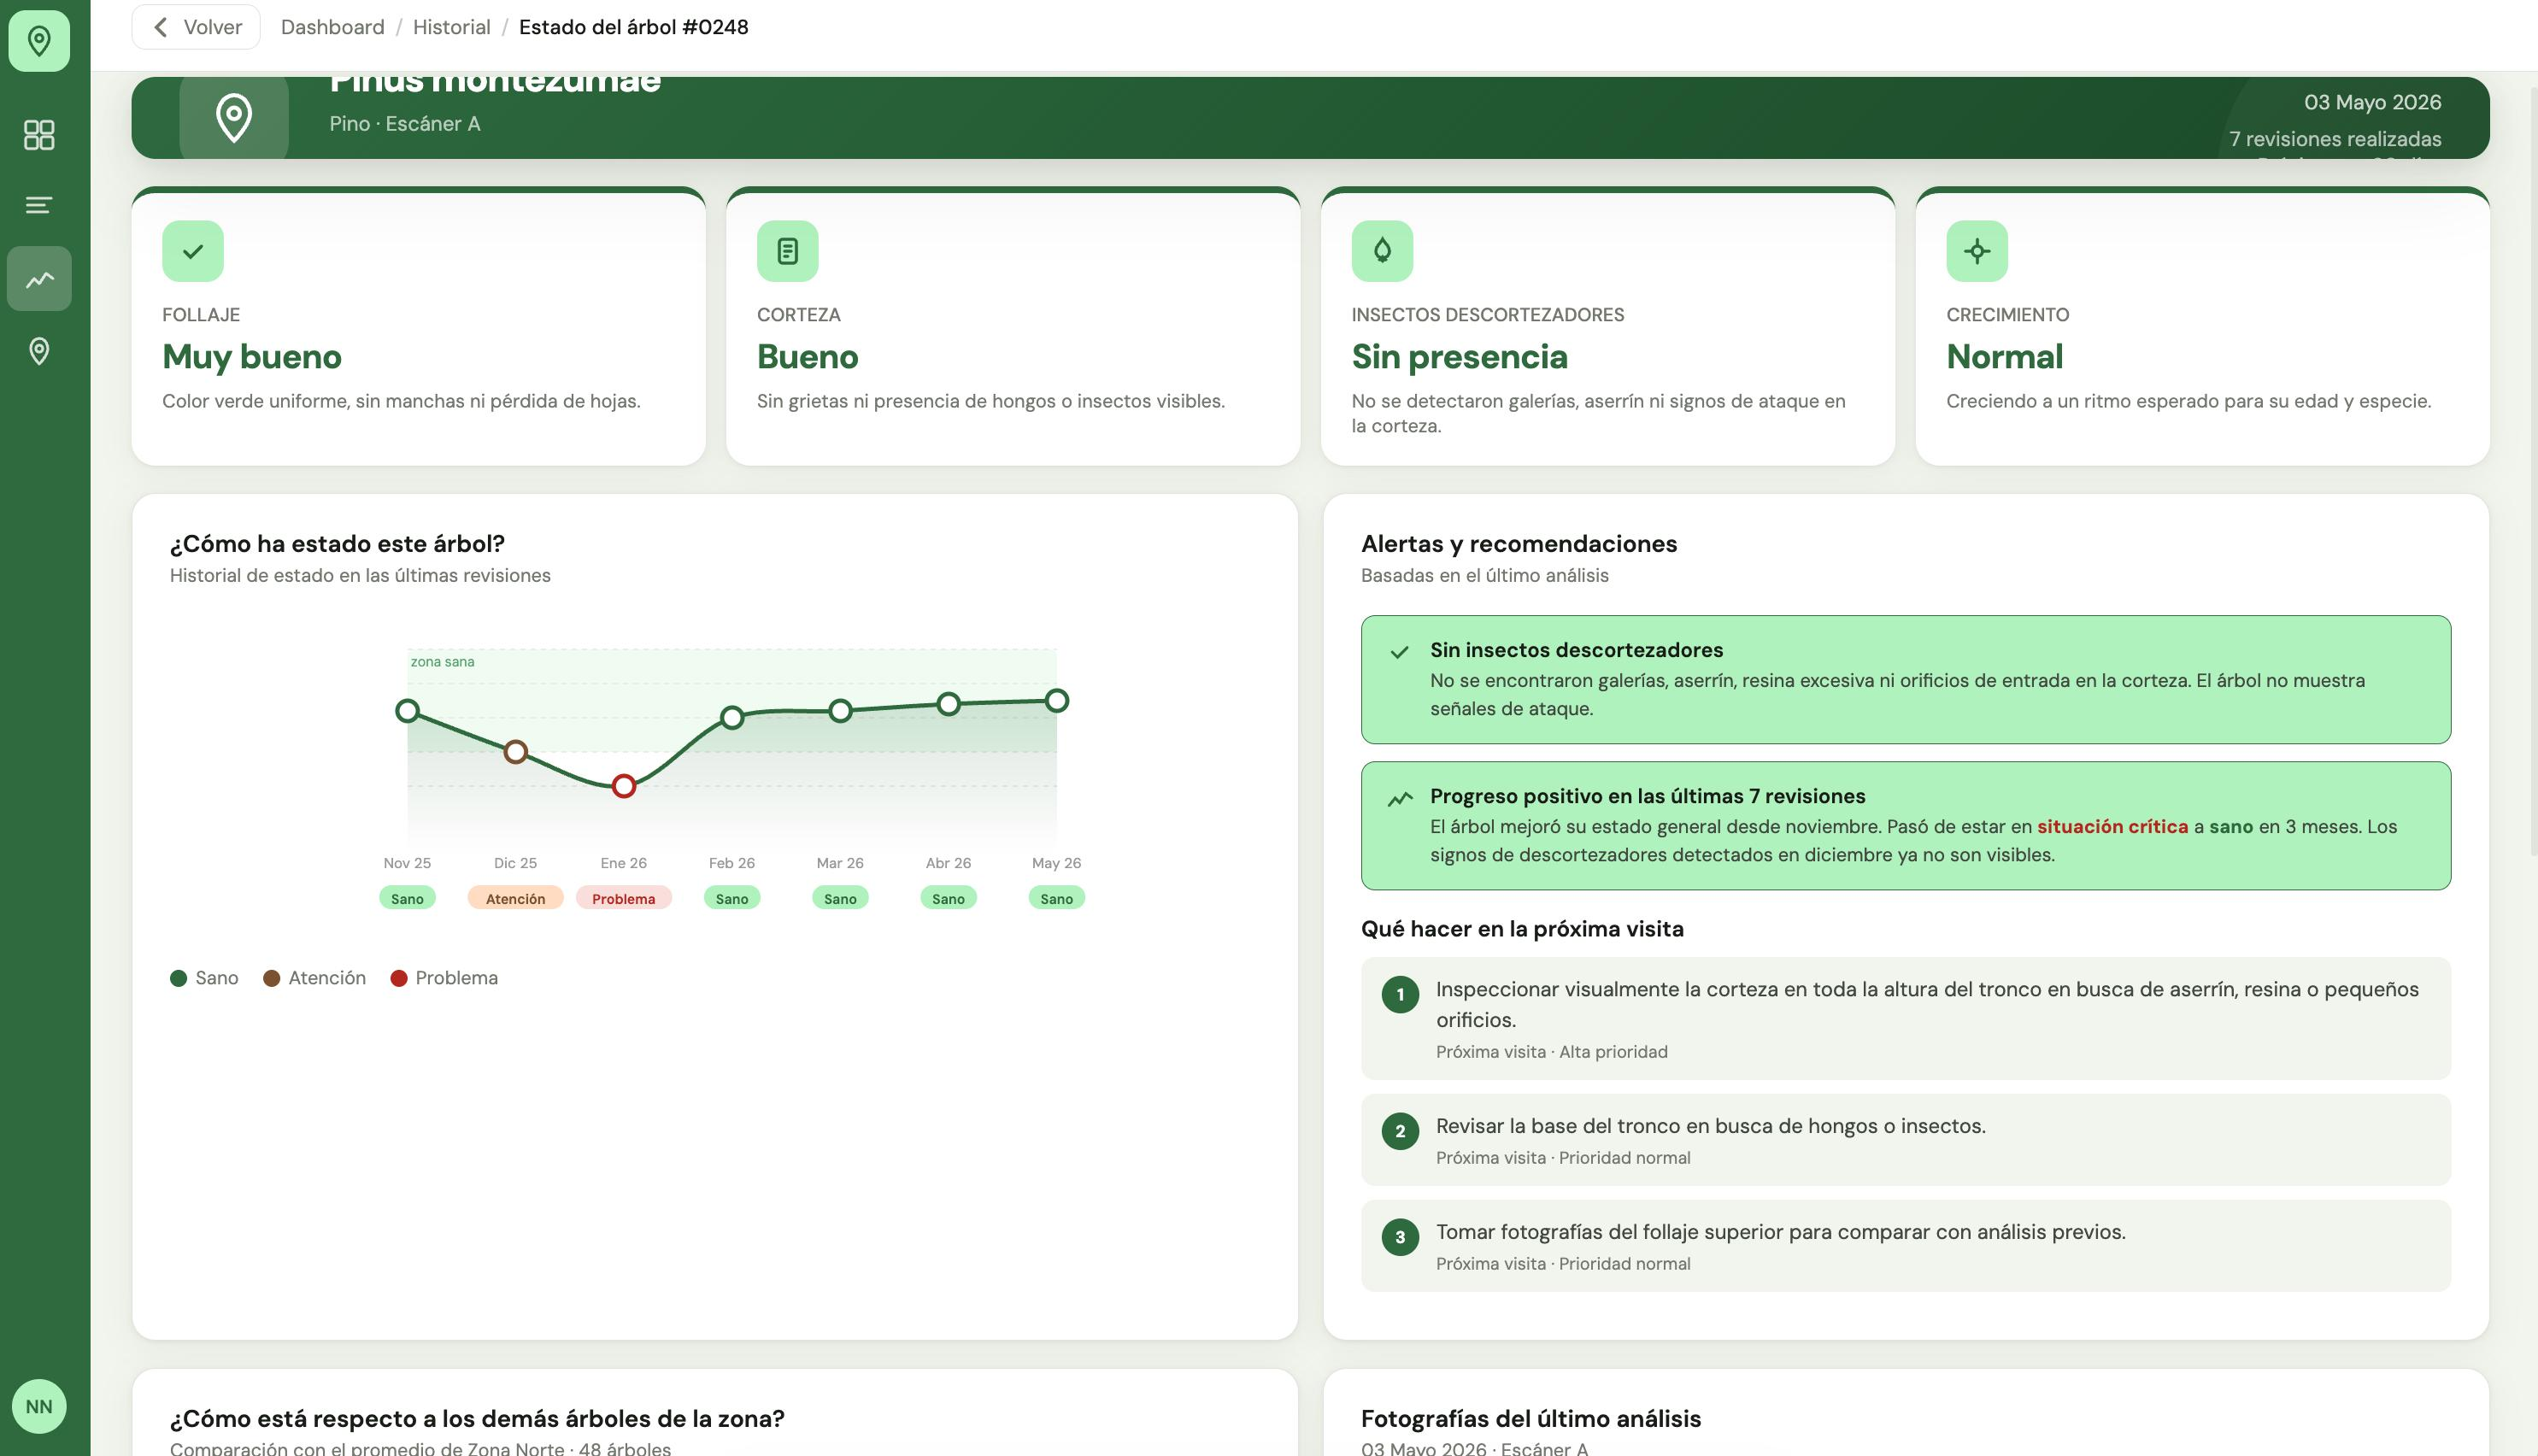
\includegraphics[width=1\textwidth]{images/Pantallas/Web/analisis.jpeg}
    \caption{Interfaces de análisis detallado y estadísticas.}
    \label{fig:web_analisis_d3}
\end{figure}

